%Centralizar verticalmente.
\newenvironment{midpage}{\vspace*{\fill}}{\vspace*{\fill}}
%Centralizar horizontalmente.
\newenvironment{midline}{\hspace*{\fill}}{\hspace*{\fill}}
\documentclass[12pts]{article}
\usepackage[utf8]{inputenc} 
\title{
	Prática de Eletrônica Digital 1 - (119466)
	\singlespacing
		Turma E (Unb - Gama)
	\singlespacing
	\begin{midpage}
	\begin {large}
		Pré-Relatório Experimento 2
		\singlespace
		Circuitos Lógicos Combinacionais
	\end {large}
	\end{midpage}
}
\date{Agosto 22, 2016}
\usepackage{indentfirst}
\usepackage{setspace}
\usepackage{verbatim}
\usepackage[pdftex]{hyperref}
\usepackage{graphicx}
\begin{document}
\maketitle	
%\vspace{100 mm}
\begin{center}

\begin{tabular}{|c|l|r|}
\hline
Nome & Matrícula & Assinatura\\
\hline
Arthur Temporim & 140016759 & \\
\hline	
Eduardo Nunes& 140056149 & \\
\hline	
\end{tabular}

\end{center}

\pagebreak

\section{Projetos e simulações}

\subsection{1.1 Análise de um Circuito Digital}

\begin{itemize}
	\item \textbf{Quantas entradas e saídas tem o circuito?}
	
	O circuito tem 3 entradas: \textbf{A,B e C}. E uma saída sendo esta: \textbf{S}.

	\item \textbf{O circuito apresenta uma porta E de três entradas. Como é possível obtê-la a partir de portas E de duas entradas? Justifique.}
	
	A partir de duas portas AND, utilizando uma para verificar os valores de duas entradas e logo em seguida uma outra para verificar o valor da primeira verificação com uma terceira entrada.
	
	\item \textbf{Apresente a tabela-verdade do circuito;}
	
	A tabela esta em um arquivo no drive.
	
	\item \textbf{Explique que este circuito faz, i.e., apresente uma possível função para o mesmo.}
	
	O circuito representado pela figura 2.1, compara os valores de 3 entradas. Se o nível de duas entradas ou mais, forem altos, então, este terá um sinal alto em sua saída.
	
	Uma possível função para este seria em uma compra para o show se o comprador tiver dois dos seguintes items: carteirinha, 1Kg de alimento e o cartão de filiação este poderá pagar a meia entrada.
	
	Uma função booleana para este circuito seria: S = AB + AC +  BC.
	
\end{itemize}

\subsection{1.2 Projeto 1}

\begin{itemize}
	\item \textbf{Diagrama}

\begin{figure}[!htb]
  \centering
  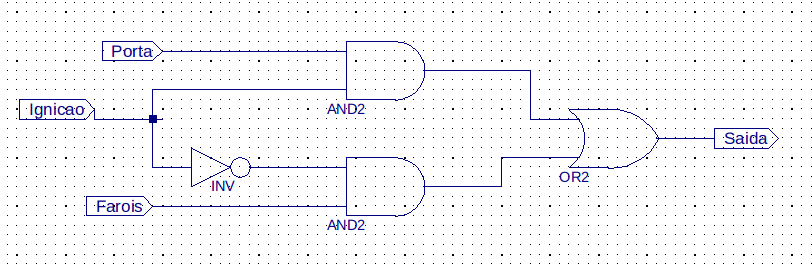
\includegraphics[scale=0.5]{imagens/diagrama01}
  \caption{Diagrama Alarme - Ise Design Suit 14.7}
  \label{figRotulo}
\end{figure}		
	
	\item \textbf{Tabela Verdade}
\begin{center}
	\begin{tabular}{|r|r|r|r|}
		\hline
		Porta & Ignição & Faróis & Saída \\
		\hline
		0 & 0 & 0 & 0 \\
		\hline
		0 & 0 & 1 & 0 \\
		\hline
		0 & 1 & 0 & 0 \\
		\hline
		0 & 1 & 1 & 1 \\
		\hline
		1 & 0 & 0 & 0 \\
		\hline
		1 & 0 & 1 & 1 \\
		\hline
		1 & 1 & 0 & 1 \\
		\hline
		1 & 1 & 1 & 1 \\
		\hline
	\end{tabular}
\end{center}

	\item \textbf{Forma de Onda}	

\begin{figure}[!htb]
  \centering
  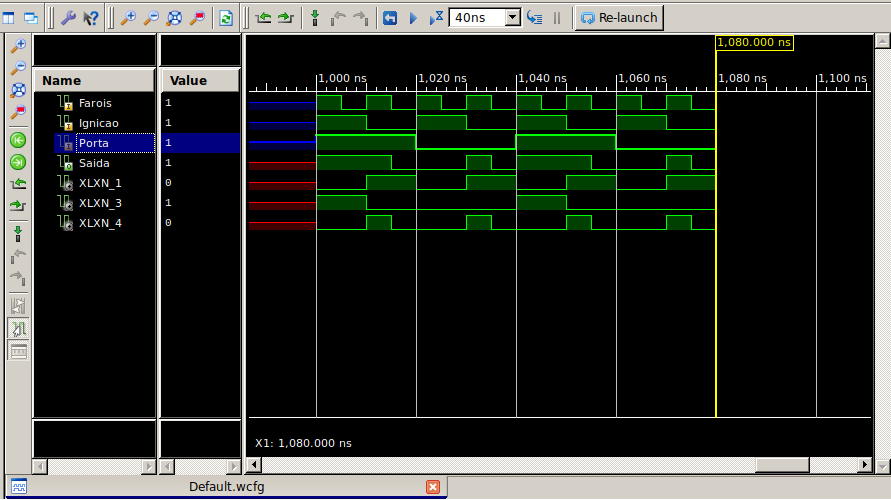
\includegraphics[scale=0.5]{imagens/projeto01}
  \caption{Forma de onda Alarme - Ise Design Suit 14.7}
  \label{figRotulo}
\end{figure}				
	
\end{itemize}

\subsection{1.2 Projeto 2}

\iffalse
\begin{itemize}
	\item \textbf{Diagrama}

\begin{figure}[!htb]
  \centering
  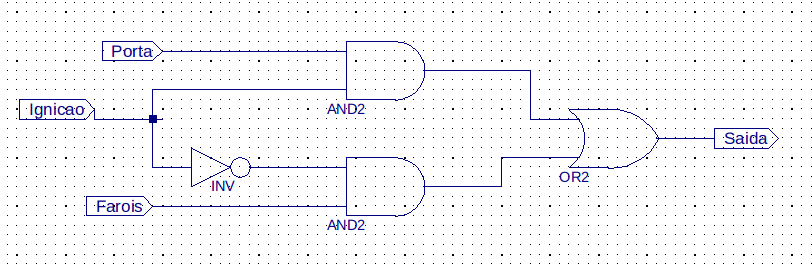
\includegraphics[scale=0.5]{imagens/diagrama01}
  \caption{Diagrama Alarme - Ise Design Suit 14.7}
  \label{figRotulo}
\end{figure}		
	
	\item \textbf{Tabela Verdade}
\begin{center}
	\begin{tabular}{|r|r|r|r|}
		\hline
		Porta & Ignição & Faróis & Saída \\
		\hline
		0 & 0 & 0 & 0 \\
		\hline
		0 & 0 & 1 & 0 \\
		\hline
		0 & 1 & 0 & 0 \\
		\hline
		0 & 1 & 1 & 1 \\
		\hline
		1 & 0 & 0 & 0 \\
		\hline
		1 & 0 & 1 & 1 \\
		\hline
		1 & 1 & 0 & 1 \\
		\hline
		1 & 1 & 1 & 1 \\
		\hline
	\end{tabular}
\end{center}

	\item \textbf{Forma de Onda}	

\begin{figure}[!htb]
  \centering
  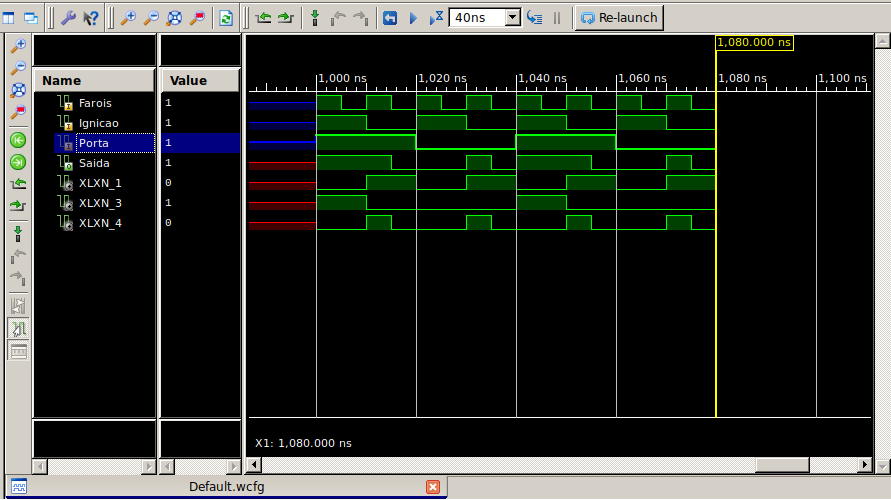
\includegraphics[scale=0.5]{imagens/projeto01}
  \caption{Forma de onda Alarme - Ise Design Suit 14.7}
  \label{figRotulo}
\end{figure}				
	
\end{itemize}

\fi

\newpage
\section{Referências Bibliográficas}

\end{document}

%Exemplo de imagem
\iffalse
\begin{figure}[!htb]
  \centering
  \includegraphics[scale=0.3	]{nome_da_imagem}
  \caption{Descrição}
  \label{figRotulo}
\end{figure}
\fi

% Exemplo de tabela.
\iffalse
\begin{tabular}{|c|r|}
\hline
Material Utilizado & Quantidade\\
\hline
Cabo Banana-Banana & 2  \\
\hline
Fios de cobre & x \\
\hline
Cabo coaxial & 3  \\
\hline
CI 74HC00   & 1 \\
\hline
CI 74LS00   & 1 \\
\hline
Protoboard & 2 \\
\hline
Fonte de tensão MPL-3305M & 1 \\
\hline	
Multímetro Digital  & 1 \\
\hline
Gerador de funçoes iCEL modelo GV-2002 & 1 \\
\hline
Osciloscopio BK 2530 & 1 \\
\hline
\end{tabular}
\singlespacing
\fi